\documentclass[12pt,a4paper]{report}

\usepackage{enumitem}
\usepackage[utf8x]{inputenc}
\usepackage[francais]{babel}
\usepackage[T1]{fontenc}
\usepackage{amsmath}
\usepackage{amsfonts}
\usepackage{amssymb}
\usepackage[square,sort,comma,numbers]{natbib}
\usepackage[colorlinks=true,linkcolor=blue]{hyperref}
\usepackage{glossaries}
\usepackage[usenames,dvipsnames]{xcolor}
\usepackage{setspace}
\usepackage{graphicx}
\usepackage{float}
\usepackage[skip=2pt,font=scriptsize]{caption}
\usepackage{listings}
\usepackage{xcolor}



\author{Nicolas JEANNE}
\title{Rapport de stage de M2}
\date{11 mars 2015}

% Mise en page des citations
\bibliographystyle{abbrvnat}
\setcitestyle{authoryear,open={(},close={)},aysep={},citesep={;}}


% formattage des entrées du glossaire
\renewcommand*{\glstextformat}[1]{\textcolor{Black}{#1}}
% création des acronymes du glossaire
\newacronym{rep}{REP}{Repeated Extragenic Palindrome}
\newacronym{bime}{BIME}{Bacterial Interspesed Mosaic Element}
\newacronym{sra}{SRA}{Sequence Read Archive}
\newacronym{ngs}{NGS}{Next Generation Sequencing}
\newacronym{sam}{SAM}{\href{http://samtools.github.io/hts-specs/SAMv1.pdf}{Sequence Alignment Map format}}
\newacronym{bam}{BAM}{Binary Alignment Map format}
\newacronym{gff}{GFF}{General Feature Format}
\newacronym{bed}{BED}{Browser Extensible Data}
\newacronym{de}{DE}{Diff\'erence d'Expression}
\newacronym{rpkm}{RPKM}{Reads Per Kilobase per Million mapped reads}
% création des entrées du glossaire
\newglossaryentry{PE}{name={Paired-end},description={Technique de séquençage haut débit consistant à réaliser les amplifications d'un fragment d'ADN en marquant l'extrémité 5' par un tag \no1 et l'extrémité 3' par un tag \no2. La distance entre les 2 tags est connue et fixe (négative ou jusqu'à 500 pb). Ceci permet lors de l'assemblage, de séquences de 35 pb par exemple, d'associer le read 1 et le read 2 grâce à la distance séparant les 2 et cela même si la séquence intermédiaire est inconnue. Si la distance est négative, il est possible d'obtenir des reads chevauchants de longueur plus importante que les 35 pb}}
\newglossaryentry{reads}{name={reads},description={Séquence nucléotidique issue d'un séquençage NGS}}
\newglossaryentry{GRanges}{name={Genomic Ranges},description={Format de stockage d'informations pour les éléments génomiques sous R. L'information minimale requise est le chromosome, les positions de départ et de fin, le sens du brin. Ces champs peuvent être suivis de méta-datas où d'autres informations libres peuvent être enregistrées}}
\newglossaryentry{chimerique}{name={alignement chim\'erique},description={L'alignement d'un read ne peut pas être représenté comme un alignement linéaire. Un alignement chimérique est représenté comme un ensemble d'alignements, par exemple lorsqu'une partie d'un read est mappé à un locus du génome et la suite à un autre locus}}
\makeglossaries

% Encadrement des figures
\floatstyle{boxed}
\restylefloat{figure}

% Configuration des liens
\hypersetup{
  colorlinks,
  citecolor=Violet,
  linkcolor=Black,
  urlcolor=Blue}

% Configuration des parties de code
\lstset{basicstyle=\small}

\begin{document}

\maketitle

\begin{onehalfspace}
\chapter*{Introduction}
En 1982, la découverte par Higgins et al. de nouveaux éléments génétiques communs dans les régions intercistroniques des opérons de Escherichia coli et Salmonella typhimurium a constitué le premier pas de la recherche sur les \gls{rep} \citep{Higgins1982}. En 1991, Gilson et al. ont mis en évidence l'organisation en clusters de ces REP \citep{Gilson1991}, ces clusters ont été caractérisés comme \gls{bime}. Chez E. coli en 1994, Bachelier et al. ont réussi à catégoriser les REP constituant les BIME en 2 types Y et Z, constituants 3 motifs Y, Z\textsuperscript{1}, Z\textsuperscript{2}  \citep{Bachellier1994}.
 
Les REP constituent une part non négligeable du génome bactérien, chez E. coli K12 ou S. typhimurium elles représentent environ 1\% de celui-ci \citep{Gilson1991}. Nous les retrouvons chez de nombreux règnes bactériens, notamment chez les pathogènes humains tels que \textit{Escherichia coli, Salmonella enterica, Neisseria meningitidis, Mycobacterium tuberculosis et Pseudomonas aeruginosa} mais également chez des pathogènes des plantes comme \textit{Agrobacterium tumefaciens} ou chez des bactéries ubiquitaires, \textit{Deinococcus radiodurans} ou \textit{Pseudomonas putida} par exemple. Les travaux précédents de l'équipe ont permis l'annotation des REP au sein du génome d'E. coli et de mettre en évidence le lien existant entre la prolifération des REP et le gène $tnpA_{REP}$ \citep{Weyder2013,Bosc2014}, ainsi que la reconstruction des états ancêtres des REP \citep{Bosc2014}.  \textcolor{red}{Le rôle exact des REP n'est pas clairement défini, des hypothèses sont avancées sur leur implication dans la régulation de l'expression des gènes, que ce soit en tant que terminateur ou comme site de reconnaissance des enzymes impliquées dans les mécanismes de la transcription.}

\section*{Caractéristiques des REP et organisations en BIME}
La taille des REP varie de 20 à 40 nucléotides, la classification Y, Z\textsuperscript{1}, Z\textsuperscript{2} est basée à la fois sur la taille de la séquence consensus de la REP ainsi que sur sa structure secondaire. Par convention, une REP en orientation inversée est nommée iREP (inversed REP) \citep{Ton-Hoang2012}. Un tétra-nucléotide caractéristique de séquence GTAC est présent à l'extrémité 5' des REP, sa séquence complémentaire est CTAC en 3' pour les iREP. Les différentes classes de REP partagent des nucléotides conservés (\autoref{fig:rep_bime}A). La structure secondaire des REP est caractérisée par sa forme en tige-boucle, le caractère palindromique permet la formation de la tige malgré un mésappariement situé dans la partie centrale de celle-ci (\autoref{fig:rep_bime}B). Pour le génome d'E. coli K-12, 93 REP ont été répertoriées comme étant uniques sur les 605 annotées par le laboratoire, les autres sont organisées par paires sous forme de BIME. Une classification a été adoptée comportant 3 entrées, les BIME-1 composées de REP Z\textsuperscript{1} et Y apparaissant en paires uniques et dans lesquelles la REP et l'iREP sont séparées par un linker de séquence longue (L) pouvant lier l'IHF (Integration Host Factor). Les BIME-2 constituées de Z\textsuperscript{2} et de Y, apparaissant en copies multiples de cette paire dont la REP et l'iREP sont séparées par un linker court (S) et une des trois séquences flanquantes (s, l ou r). La troisième catégorie est constituée des BIME dites atypiques qui sont des chimères de BIME-1 et BIME-2, comportant différentes combinaisons de Y, Z\textsuperscript{1}, Z\textsuperscript{2}, S, L, s, l et r. Tout comme les BIME-2, nous les retrouvons sous forme de copies multiples (\autoref{fig:rep_bime}C). Les REP peuvent former des structures secondaires avec elles-même, mais également entre elles lorsqu'elles sont organisées sous forme de BIME (\autoref{fig:malEF_rep}).

\begin{figure}[ht]
\centerline{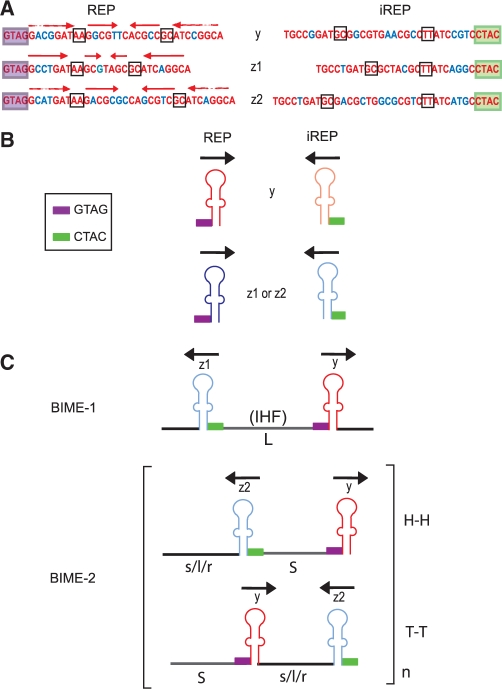
\includegraphics[scale=1.8]{figures/rep_bime.jpg}}
\caption{\textbf{REP et BIME chez Escherichia coli. (A)} Séquences consensus Y, Z\textsuperscript{1} et Z\textsuperscript{2} des REP. Le tétra-nucléotide conservé GTAC est encadré en violet, le complémentaire conservé CTAC est encadré en vert, les flèches rouges situent les zones d'appariement de la tige et les positions encadrées en noir sont les zones de mésappariement. Les positions conservées parmi les classes de REP sont en rouge, les positions variables en bleu. \textbf{(B)} Structure secondaire des REP. Les rectangles violets et verts représentent respectivement les tétra-nucléotides conservés GTAC pour les REP et CTAC pour les iREP. Les flèches noires indiquent l'orientation des REP. \textbf{(C)} Structures des BIME-1 et BIME-2. Les BIME-1 sont composées de REP et de iREP Y et Z\textsuperscript{1} séparées par un linker de séquence longue (L), les BIME-2 sont composées de Y et Z\textsuperscript{2}, de linker courts (S) et de séquences séparatrices s, l ou r. H-H et T-T dénotent respectivement une organisation tête à tête et queue à queue des REP. \citep{Ton-Hoang2012}.}
\label{fig:rep_bime} 
\end{figure}


\begin{figure}[ht]
\centerline{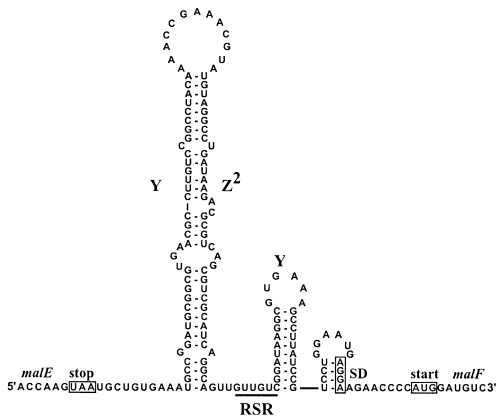
\includegraphics[scale=0.5]{figures/malEF_rep.png}}
\caption{\textbf{Structure ARN des REP au sein de l’opéron malEFG.} Y, Z\textsuperscript{2} et Y indiquent la séquence des REP dans l'espace inter-génique de malE-malF. Bien que Y et Z\textsuperscript{2} puissent former des structures tige-boucles par elles mêmes, elles s'apparient ensemble pour former une région étendue en grande partie à double brin (70\% des nucléotides sont appariés). La séquence affichée provient du génome d'E. coli K12. La région REP-stabilized RNA (RSR) indique l'extrémité 3′ du messager malE mature, qui s'étend de 3 à 9 nucléotides depuis la base de la tige-boucle formée par Y et Z\textsuperscript{2}. Les codons STOP de  malE et START de malF sont encadrés. SD représente la séquence Shine–Dalgarno nécessaire à l'initiation de la traduction de malF. \citep{Khemici2004}.}
\label{fig:malEF_rep} 
\end{figure}


\section*{Propriétés associées aux REP}
La littérature décrit de nombreuses fonctions associées aux REP, mais certaines d'entre elles restent encore peu étudiées. Les REP ont été décrite comme jouant un rôle dans les événements de recombinaisons homologues \citep{Kofoid2003}. Les BIME ont été décrites comme des sites privilégiés pour l'insertion de séquences d'ADN mobiles comme certaines familles d'IS (Insertion Sequence) \citep{Bachellier1997,Clement1999,Choi2003,Tobes2005}. Lorsqu'elles sont transcrites, les REP joueraient un rôle dans la stabilisation de l'ARNm grâce à leur structure en tige-boucle \citep{Newbury1987,Espeli2001,Khemici2004,Aguena2009}, la terminaison de la transcription \citep{Gilson1986} et le contrôle de la traduction \citep{Stern1988}. Au niveau de l'ADN, les REP sont capables de lier plusieurs facteurs protéiques tels que l'ADN Gyrase \citep{Espeli1997} et l'ADN polymérase \citep{Gilson1990}. Plus spécifiquement, la BIME-1 peut lier l'IHF sur son linker \citep{Boccard1993} qui peut être notamment responsable de l'initiation de la transcription et d’événements de recombinaisons sites spécifiques \citep{Goosen1995}.

\section*{Transcription chez E. coli}

\subsection*{Stabilité des ARN}

\chapter*{Matériel \& Méthodes}

\section*{Données}
Les données que nous avons exploité sont issues des expériences d'évolution adaptatives en laboratoire visant à découvrir l'émergence de mutations clés permettant la croissance rapide d'E. coli K-12 MG1655 sur un medium pauvre en glucose \citep{Lacroix2014}. Ces données ont été choisies car elles proviennent d'expériences de RNA-Seq comportant un nombre non négligeable de réplicats (9) pour la condition de croissance en milieu pauvre en glucose (ALE) et 2 réplicats pour le Wild Type (WT) . Il s'agit de données \gls{ngs} publiques, accessibles sur le base de données \href{http://www.ncbi.nlm.nih.gov/geo/query/acc.cgi?acc=GSE61327}{GEO} (Gene Expression Omnibus) du NCBI au format \gls{sra}, séquencées sur Illumina MiSeq à partir d'ARN total extrait des cultures d'E. coli et rétro-transcrit en cDNA. La librairie a été conçue en \gls{PE} et brin spécifique en utilisant la méthode dUTP \citep{Levin2010}. Grâce au \href{http://www.ncbi.nlm.nih.gov/books/NBK158900/#SRA_download.how_do_i_use_the_sra_toolki}{SRA toolkit} et à la commande \texttt{fastq-dump}, elles sont décompressées au format \texttt{fastq}. Un contrôle de qualité a été effectué afin d'inspecter les séquences grâce au logiciel \texttt{fastqc}. Les 2 WT et 8 ALE ont été validés puisque disposant d'une qualité de séquence par base supérieure à 30 pour des \gls{reads} de 62 pb. Seul le fichier \texttt{SRR1573441.fastq} a été rejeté car la longueur des reads allait de 35 à 502 pb avec des scores de qualités très variables.

\section*{Alignement des reads}
Les reads ont été alignés grâce au logiciel \href{http://bio-bwa.sourceforge.net/}{BWA} sur le génome d'E. coli \href{http://www.ncbi.nlm.nih.gov/nuccore/NC_000913.2}{NC\_000913.2} qui est le génome utilisé pour annoter les REP au laboratoire.  Le logiciel BWA propose 3 algorithmes distincts, BWA-backtrack, BWA-SW et BWA-MEM. Pour chacun de ces alignements, il est nécessaire de disposer d'une séquence de référence indexée, obtenue par la commande \texttt{bwa index NC\_000913.2.fasta}. 
L'algorithme que nous avons sélectionné est le MEM (Maximal Exact Matches) car il s'agit du plus récemment développé. Il reprend les mêmes principes que BWA-SW (utilisation de la programmation dynamique pour trouver les seeds en autorisant les mismatchs et les gaps. Il n'étend les alignements des seeds que lorsque ceux-ci ont peu d'occurrences sur le génome de référence, cela permet de diminuer le temps d'alignement en éliminant les extensions des séquences très répétées) mais en utilisant le seeding avec des MEM, puis il réalise l'extension avec les autorisations de mismatchs et de gaps.
\lstset{language=sh, commentstyle=\color{ForestGreen}} 
\begin{lstlisting}[frame=single]
# Alignement avec l'algorithme MEM de BWA
bwa mem ref.fasta file.fastq > aln.sam
\end{lstlisting}
Le fichier d'alignement généré est au format \texttt{\gls{sam}}, afin de poursuivre l'analyse il doit être convertit au format binaire \texttt{\gls{bam}}, des critères de qualité sont appliqués. Seules les séquences possédant une qualité de mapping > 30 et n'étant pas taggées comme \gls{chimerique} sont conservées. Cette opération a aussi le mérite de compresser l'information et de gagner de l'espace de stockage. Les séquences vont ensuite être triées par position génomique.

Finalement, le fichier BAM trié doit être indexé pour être visualisable sur un Genome Browser. Les outils utilisés sont compris dans la suite des \href{http://samtools.sourceforge.net/samtools.shtml}{samtools}.
\lstset{language=sh, commentstyle=\color{ForestGreen}}  
\begin{lstlisting}[frame=single]
# Conversion du SAM en BAM et application des filtres
# de qualite.
samtools view -Sbh -q 30 -F 2048 aln.sam > aln.bam

# Tri en fonction des positions genomiques
samtools sort aln.bam aln_sorted

# Indexation du fichier d'alignement
samtools index aln_sorted.bam
\end{lstlisting}

Pour les besoins ultérieurs de l'analyse, les réplicats d'une même condition sont fusionnés en un seul fichier.
\lstset{language=sh, commentstyle=\color{ForestGreen}}  
\begin{lstlisting}[frame=single]
# Fusion des replicats.
samtools merge merged.bam aln_sorted_1.bam \
aln_sorted_2.bam aln_sorted_3.bam
\end{lstlisting}

\section*{Préparation des fichiers de référence}
Le fichier \texttt{\gls{gff}} d'annotation du génome a été généré par un script Perl à partir du fichier \href{http://www.ncbi.nlm.nih.gov/nuccore/NC_000913.2}{GenBank}. Les fichiers répertoriant les opérons, les promoteurs, les terminateurs de transcription (source \href{http://regulondb.ccg.unam.mx/}{RegulonDB}) ainsi que les REP et BIME (source laboratoire) ont été transformés au format \texttt{\gls{bed}} grâce à des scripts Python.
Ces changements de format permettent de travailler aisément avec la suite de logiciels \href{http://bedtools.readthedocs.org/en/latest/}{BEDtools} pour la recherche d'intersections, de positions proches ou de couverture de reads. Ces outils ont généré les fichiers BED nécessaires à la suite de l'analyse tel que celui des positions génomiques des opérons contenant des REP, celui des REP, celui des gènes contenus dans des opérons bordant une REP, celui des BIME et celui de la couverture sur les régions contenant des BIME.

\section*{Visualisation du mapping}
L'alignement des reads et le mapping sur le génome de référence de E. coli sont visualisés grâce au genome browser \href{https://www.broadinstitute.org/igv/}{IGV} (\autoref{fig:igv}).
\begin{figure}[ht]
\centerline{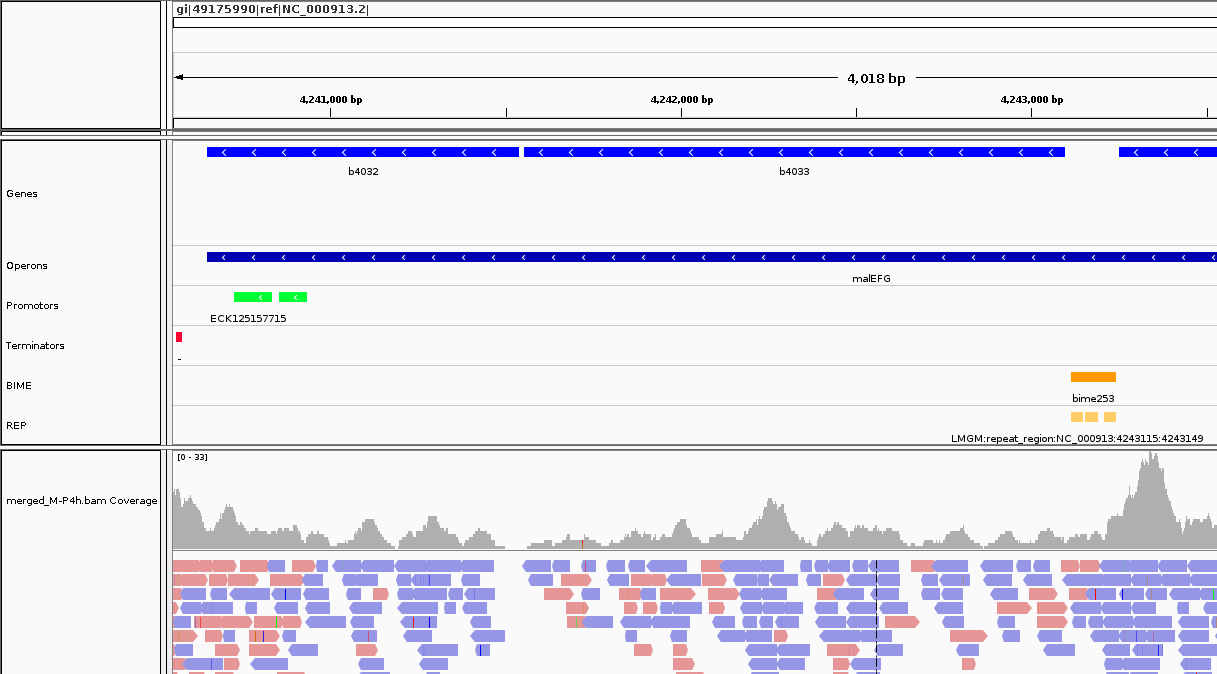
\includegraphics[scale=0.246]{figures/igv_snapshot.png}}
\caption{\textbf{Visualisation du mapping de l'opéron malEFG sur IGV.} Les premières pistes représentent les positions et orientations des gènes, des opérons, la présence de promoteurs et de terminateurs, ainsi que la position des BIME et des REP qui composent les BIME. Les 2 pistes suivantes affichent la couverture des fichiers BAM fusionnés de la région visualisée (histogramme gris) et l'alignement des reads (flèches pleines rouges et bleues). La couleur bleue sur cette piste indique un alignement en anti-sens et la couleur rouge, un alignement en sens.}
\label{fig:igv} 
\end{figure}

Il est important de noter que la couverture au long du génome n'est pas uniforme, ni même sur les gènes, car nous observons la présence de nombreuses vallées et pics. Ce phénomène s'explique par plusieurs raisons techniques \citep{Li2013}. Premièrement, les méthodes de fragmentation des protocoles de préparation des bibliothèques amenant un biais en cassant ou dégradant certaines séquences. Le second biais possible est amené par le Random Priming lors de l'étape de rétro-transcription pouvant préférentiellement transcrire certaines séquences. Troisième point, les ligases peuvent lier préférentiellement les adaptateurs à certaines séquences. Quatrième point, l'amplification de la PCR est bien connue pour introduire des biais dépendant de la proportion en GC des séquences. Le dernier point, étudié sur le séquençage Illumina, implique des interférences spécifiques aux séquences lors du processus d'élongation pendant le séquençage générés par des schémas particuliers du template produisant des repliements du brin d'ADN et altérant l'affinité des enzymes \citep{Nakamura2011}.

\section*{Analyse statistique}
Pour réaliser nos analyses, nous nous sommes inspirés de la méthodologie employée en RNA-Seq pour l'étude de \gls{de}. Il est important de noter qu'une différence importante existe avec notre approche, car nous ne nous intéressons pas à une DE pour un m\^eme gène dans différentes conditions mais plut\^ot à la \emph{DE entre deux gènes pour lesquels ont pourrait supposer un profil d'expression similaire dans une même condition}, comme c'est le cas dans les opérons par exemple.
L'analyse statistique a été menée sur le logiciel R.

\subsection*{Création de la table de comptages et normalisation}
Afin d'obtenir des résultats de comptage par transcrit et ainsi estimer l'expression, nous avons utilisé le package Bioconductor easyRNASeq \citep{Delhomme2012}. Les annotations du génome d'E. coli touchant aux transcrits sont extraites à partir du fichier GFF et stockées sous forme d'une base de données. Cela a nécessité une manipulation préalable du fichier GFF, en effet les opérons récupérés sur RegulonDB sont composés à la fois de gènes dont les transcrits sont annotés ARNm, ARNt et ARNr. Seul les gènes dont le transcrit est annoté ARNm est pris en compte par le package easyRNASeq, donc pour ne pas avoir d'erreur dans l'analyse, nous avons transformé les annotations ARNt et ARNr en ARNm.
La liste des transcrits par gènes est ensuite extraites pour un total de 4605 éléments. La couverture par transcrit est ensuite calculée pour chaque fichier BAM, le résultat est obtenu en réalisant l'union des positions extraites de la liste des transcrits et des positions des reads extraites des fichiers BAM qui auront été préalablement transformées au format \gls{GRanges} (GRanges)  \citep{Lawrence2013}. Une table de comptage est alors produite, les transcrits figurant en ligne et les fichiers BAM en colonnes (\autoref{fig:easyRNAseq}).

\begin{figure}[ht]
\centerline{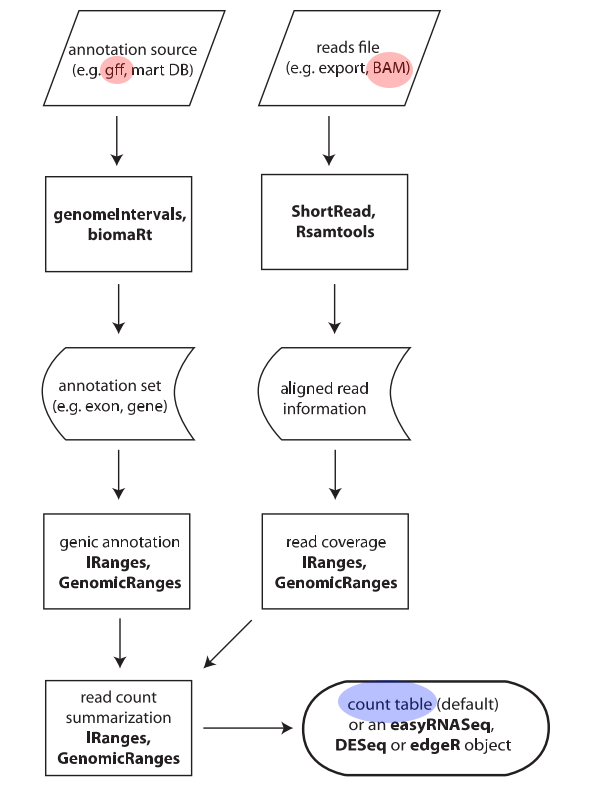
\includegraphics[scale=0.3]{figures/easyRNASeq.png}}
\caption{\textbf{easyRNASeq : création d'une table de comptage.} Processus de création de la table de comptage grâce à l'union des intervalles génomiques. Les formats d'entrées de notre analyse sont surlignés en rouge, le format de sortie en bleu \citep{Delhomme2012}.}
\label{fig:easyRNAseq} 
\end{figure}

Les résultats de comptages doivent ensuite être normalisés afin de permettre la comparaison de l'expression des gènes et des régions génomiques d'intérêt. Notre choix s'est porté sur la méthode du \gls{rpkm} \citep{Mortazavi2008} :

\[RPKM = Nb.~reads~transcrit~*~\frac{1000~bases~*~10^6}{Nb.~total~reads~*~Taille~du~transcrit}\]

Le RPKM reflète la concentration molaire du transcrit en normalisant par la longueur du brin d'ARN et le nombre de reads de la bibliothèque. Cette normalisation est soumise à critique à juste titre \citep{Dillies2013} car elle induit un biais de lors d'une analyse de DE dans le cas de gènes fortement exprimés dans un condition par rapport aux autres. Comme nous ne nous situons pas dans le cadre d'une analyse différentielle sur plusieurs conditions, mais que nous comparons des réplicats d'une même condition, nous pouvons appliquer cette normalisation.

Une analyse en composante principale est réalisée sur ces données normalisées afin de vérifier l'homogénéité des réplicats et les taux d'expressions moyens des gènes et des BIME sont visualisés sous forme de BoxPlot.

\subsection*{Différence d'expression dans les opérons contenant des BIME}
L'hypothèse privilégiée ici est que les gènes appartenant à un opéron vont être exprimés à un taux similaire, la question qui se pose est de savoir si la présence d'une BIME entre 2 gènes d'un opéron va avoir un impact sur la transcription d'un des gènes. Dans ce cadre, les opérons contenant des BIME sont sélectionnés et l'expression des 2 gènes de l'opéron entourant la BIME recueillie. Si l'expérience contient au moins 5 réplicats, un test non paramétrique de rangs de Wilcoxon est effectué dont l'hypothèse nulle est qu'il n'existe pas de différence d'expression entre les 2 gènes. La p-value significative étant fixée à 0.01. Dans le cas où le nombre de réplicats est inférieur à 5, un test de Student est réalisé avec la même p-value significative.

Pour les gènes dont le test est significatif, deux représentations graphiques sont générées. La 1\up{ère} est un schéma décrivant les taux d'expression des gènes de l'opéron ainsi que la position de la BIME. La 2\up{nde} est une représentation de la couverture sur l'opéron par rapport à l'organisation génomique de celui ci ainsi que la catégorisation des REP formant la BIME. Deux fichiers au format \texttt{CSV} sont créés, l'un pour les gènes où nous observons un différence d'expression significative, le second pour les autres cas.

\subsection*{Analyse par profil d'expression}
Nous avons créé un outil analysant qui réalise un test de corrélation entre les profils d'expression des régions contenant des BIME et un profil modèle de changement d'expression en nous inspirant d'une technique mise au point pour la prédiction d'opérons dans les génomes bactériens \citep{Fortino2014}. Pour cela, il a d'abord été nécessaire de délimiter nos régions d'intérêt. Celles-ci se modélisent par la présence du 1\up{er} gène, de la 1\up{ère} région inter-génique, de la BIME, de la 2\up{nde} région inter-génique et du 2\up{nd} gène. Une fois ces régions extraites, le calcul de la couverture base par base a été réalisé à l'aide des BEDtools :
\lstset{language=sh, commentstyle=\color{ForestGreen}}  
\begin{lstlisting}[frame=single]
# Couverture base par base.
bedtools coverage -abam merged.bam -b regionOfInterest.bed \
-d > unsorted_cov_perBase.bed

# Tri en fonction de la position genomique 
# puis de la position des bases dans chaque transcrit
sort -k2 -k7 -n unsorted_cov_perBase.bed | uniq > \
cov_perBase_strandToFix.bed

# Remplacement des '.' par des '*' dans la colonne
# des brins pour l'utilisation sous R
awk 'BEGIN{OFS = "\t"} {gsub(/\./,"*",$6); print }' \
cov_perBase_strandToFix.bed > cov_perBase.bed
\end{lstlisting}
Le cœur de cette méthode consiste déplacer une fenêtre glissante parcourant base à base la région d'intérêt définie ci-dessus en réalisant des tests de corrélation entre le profil d'expression réel et un profil d'expression simulé par un vecteur contenant un nombre égal de 0 et de 1 (si l'on cherche une croissance d'expression en sens ou une décroissance d'expression en anti-sens, e.g: 000111), ou de 1 et de 0 (dans le cas d'une décroissance en sens et d'une croissance en anti-sens, e.g: 111000). Les moyennes d'expression sont récupérées sur les parties gauche et droite de la fenêtre pour dans un premier temps filtrer les données. Le $Log_2$ du rapport de ces moyennes doit être supérieur à un seuil, si ce 1\up{er} filtre est passé, la corrélation entre le profil réel et celui simulé est calculée et doit être supérieure à un seuil avec une p-valeur significative (\autoref{fig:profil}). 

\begin{figure}[ht]
\centerline{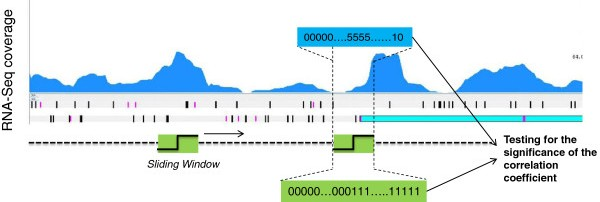
\includegraphics[scale=0.6]{figures/profil.jpg}}
\caption{\textbf{Recherche de corrélation sur des profils d'expression.} La fenêtre glissante (en vert) parcourt la région d'intérêt et pour chaque déplacement une corrélation est calculée entre le vecteur du profil d'expression obtenu par RNAseq (en bleu) et celui simulé par le vecteur de 0 et de 1 (en vert) \citep{Fortino2014}.}
\label{fig:profil} 
\end{figure}

Les seuils que nous avons fixés sont les suivants : 
\begin{itemize}[label=$\bullet$]
\item fenêtre glissante de 300 bases
\item $log_2(\frac{\overline{couverture~droite}~+~1}{\overline{couverture~gauche}~+~1})~\geq~1$ pour un profil \_\_\_|\^{ }\^{ }\^{ }
\item $log_2(\frac{\overline{couverture~gauche}~+~1}{\overline{couverture~droite}~+~1})~\geq~1$ pour un profil \^{ }\^{ }\^{ }|\_\_\_
\item une corrélation > 0.7
\item une p-valeur du test de corrélation $< 10^7$
\end{itemize}

Sur un ensemble de positions consécutives dont les corrélations sont significatives et sont situées sur l'espace génomique de la BIME (étendu de 40 pb de chaque côté), celle dont la corrélation est la plus élevée sera définie comme position de changement d'expression. Deux types de fichiers sont générés au format \texttt{bedgraph} pour une visualisation sur un Genome Browser, le premier sous forme d'histogramme représentant les couvertures moyennes des deux parties de la fenêtre, le second représentant l'évolution de la corrélation sur la zone (\autoref{fig:igv_profil}). Une visualisation des niveaux d'expression des 2 gènes et de la BIME est également générée sous forme d'histogrammes avec les informations de sens et du type de la BIME. Finalement des fichiers au format \texttt{CSV} recueillent toutes les informations de l'analyse.

\begin{figure}[ht]
\centerline{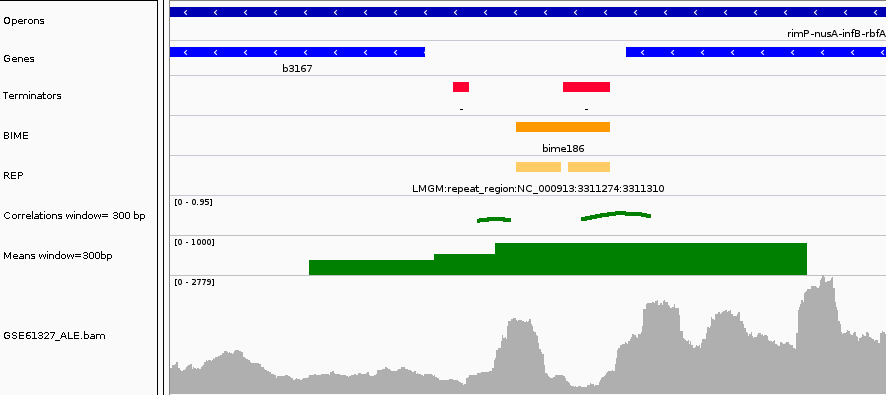
\includegraphics[scale=0.246]{figures/igv_profil.png}}
\caption{\textbf{Visualisation des changements d'expression obtenus par la méthode de corrélation des profils.} La position de la BIME est représentée en orange, l'histogramme à 2 colonnes en vert montre les profils d'expression moyens de chaque moitié de la fenêtre et la courbe en points verts indique l'évolution de la corrélation sur cette zone. Dans cet exemple, ce changement d'expression peut se traduire par une augmentation en sens ou une diminution en anti-sens}
\label{fig:igv_profil} 
\end{figure}

\subsection*{Analyse par segmentation}












\end{onehalfspace}


% affichage du glossaire
\printglossary[type=\acronymtype ,title=Glossaire]

%\bibliographystyle{unsrtnat}
\bibliography{biblio_rapport}

\end{document}